\documentclass[xcolor=table,aspectratio=169]{beamer}
\usetheme{PaloAlto}
\usecolortheme{seahorse}
%好看的颜色主题:crane、dove、rose、seahorse、wolverine
\usepackage{biblatex}
%\bibliographystyle{apalike}
\bibliography{biblatex}

%重定义、新定义
\newtheorem{thm}{定理}
\renewcommand\proofname{证明}

\usepackage[UTF8,noindent]{ctex} %ctex只引入必要的中文,ctexcap还会翻译图表等环境名称; noindent阻止ctex引入的段前缩进,这也是备案么人文档类的默认设置,幻灯片的段落不使用首行缩进。
\graphicspath{{figures/}}
\logo{\includegraphics[scale=0.2]{title}} % 校徽、公司商标
\usepackage{tikz}
%\usepackage{multimedia}  % 插入视频、音频,只能PDFlatex编译
\usepackage{media9} %可xelatex编译,支持各类媒体和3D对象,各种编译引擎和输出驱动

\usepackage{tdclock} %插入日期和时间,可用来演讲中计时



%\usepackage{fragile}  %代码文本化




\title[标题短形式]{标题名} % 短形式可能会出现在帧的顶部或底部
\subtitle{副标题}
\author{作者}
\institute{机构、学院}
\date{2019年12月1日}  %不设置则为当前日期
%\titlegraphic{标题图形} %设置标题图形,通常不设置。
% 设置PDF说明信息中的主题和关键字。
\subject{勾股定理} 
\keywords{勾股定理,历史}

\begin{document}
	
\begin{frame}[plain] % frame表示一帧
%    \maketitle
\titlepage  
\end{frame}

\begin{frame}{目录}
	\tableofcontents  %在当前帧生成目录,添加pausesections选项以动态显示
\end{frame}

\section{节标题}  %分节
\begin{frame}{帧标题}{帧小标题}
这是简单的一帧。
%	\frametitle{标题}
%    \framesubtitle{小标题}
\end{frame}



\section{列表环境} 
%\part{引言}  % 与titlepage类似,可在一帧中产生文档某部分的标题
%\begin{frame}
%	\partpage
%\end{frame}
\begin{frame}{古中国数学}{定理发现}
中国在3000多年前就知道勾股数的概念,比古希腊更早一些。

《周髀算经》的记载:
\begin{itemize} % 列表环境
	\item 公元前11世纪,商高答周公问:
	\begin{quote}  % 引用环境
		勾广三,股修四,径隅五。
	\end{quote}
    \item 又载公元前7--6世纪,\cite{__2000}陈子答荣方问,表述了勾股定理的\cite{brown_long-term_2010}一般形式:
    \begin{quote}
    	若求邪至日者,以日下为勾,日高为股,并而开方除之,得邪至日。
    \end{quote}
\end{itemize}
\end{frame}

\section{定理与区块}
\begin{frame}
	在beamer中,已经预定义了许多定理类环境:theorem、corollary、definition、definitions、fact、example以及examples,都是以英文名称给出,beamer调用amsthm宏包,可用proof证明环境。不过我们需要中文定理环境,则可以用newtheorem另行定义。
\end{frame}
\begin{frame}{现代叙述}
\begin{thm}[勾股定理]
	直角三角形斜边的平方等于两直角边的平方和。
	\begin{center}
		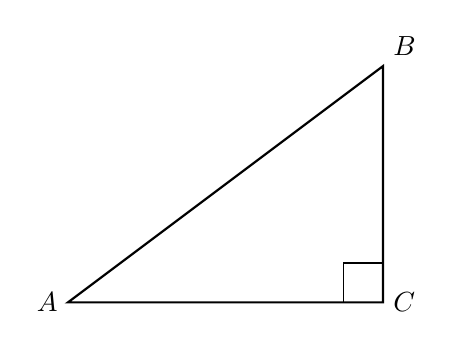
\begin{tikzpicture}
		  \draw[thick] (0,0) node[left] {$A$}
		  -- (4,0) node[right] {$C$}
		  -- (4,3) node[above right] {$B$} -- cycle;
		  \draw (3.5,0) |- (4,0.5);
		\end{tikzpicture}
	\end{center}
\end{thm}

\end{frame}
\begin{frame}
	\begin{block}{块标题}
		$$a^2+b^2=c^2$$
	\end{block}
	block、alertblock和exampleblock环境就是beamer定义的三种区块环境,它们除了使用的配色不同外,用法和结果都大致相同。
\end{frame}


\section{插入图片}
\begin{frame}
完整的证明鉴于三国时(公元3世纪)赵爽对《周髀算经》的注释。
\begin{figure}
	\centering 
	\includegraphics[height=0.4\textheight]{library}
	\caption{赵爽的炫图可给出勾股定理的一个富于对称美的证明}
\end{figure}
\end{frame}

\section{插入表格}
\begin{frame}
\rowcolors{2}{yellow}{blue}
\centering
\begin{tabular}{rrr}
	\rowcolor{red} 直角边 $a$ &直角边 $b$ & 斜边 $c$\\
	3 & 4 & 5 \\
	5 & 12 & 13\\
	7 & 24 & 25\\
	8 & 15 & 17\\
\end{tabular}
\end{frame}

\section{风格主题的选择}
\begin{frame}
beamer提供了二十多中不同风格的幻灯片主题,可以使用usetheme命令选择。\\
预定义的主题有:default、AnnArbor、Antibes、Bergen、Berkeley、Berlin、Boadilla、boxes、CambridgeUS、Copenhagen、Darmstadt、Dresden、Frankfurt、Goettingen、Hannover、Ilmenau、JuanLesPins、Luebeck、Madrid、Malmoe、Marburg、Montpellier、PaloAlto、Pittsburgh、Rochester、Singapore、Szeged、Warsaw等。

实际上,beamer主题是由不同的内部主题(inner theme)、外部主题(outer theme)、色彩主题(color theme)、字体主题(font theme)等组合而成的,可以分别使用useinnertheme、useoutertheme、usecolortheme、usefonttheme选择。

\end{frame}
\begin{frame}
	\begin{itemize}
		\item 内部主题:default、circles、rectangles、rounded、inmargin等
		\item 外部主题:default、infolines、miniframes、smoothbars、sidebar、split、shadow、tree、smoothtree等
		\item 色彩主题:default、albatross、beaver、beetle、crane、dolphin、dove、fly、lily、orchid、rose、seagull、seahorse、sidebartab、structure、whale、wolverino等
		\item 字体主题:default、professionalfonts、serif、structurebold、structureitalicserif、structuresmallcpsserif等
	\end{itemize}
\end{frame}

\section{参考文献}
\begin{frame}{参考文献}
%\bibliographystyle{apalike} % 提供基本的作者年代引用方式
	\printbibliography
\end{frame}
\begin{frame}{文献引用}
	这是高娜德\cite{__2000}所写的,约翰逊\cite{brown_long-term_2010}完善的。
\end{frame}

\section{动态演示}
\begin{frame}{不显示的内容占用原来位置}
% 使用onslide时不显示的内容还占用原来的位置
	\onslide<1>{只有第1步}
	\onslide<2->{第2步之后}
	\onslide<1,3>{第3步}
\end{frame}
\begin{frame}{没有占用,内容代替}
	计数:\only<1>{1} \only<2>{2} \only<3>{3} \only<4>{4}
	\onslide<5> 数完了。
\end{frame}
\begin{frame}
	\begin{itemize}
		\item<1-> 开始显示
		\item<3-> 最后显示
		\item<2-> 然后显示
	\end{itemize}
\end{frame}
\begin{frame}{快速计数}
	使用加号+就类似使用了pause,可避免手工计数,item<+->等价于item<1->,item<2->,item<3->···。可在enumerate或itemize环境后加[<+->]。
	\begin{itemize}[<+->]
		\item 开始显示
		\item 其次显示
		\item 最后显示
	\end{itemize}
\end{frame}
\begin{frame}
structure和alert命令用于指定的步骤设置高亮,前者使用幻灯片中结构的色彩,后者使用更鲜明的警告色彩(一般是红色)。
	\begin{itemize}
		\item<+-| alert@+> 公元前6世纪,毕达哥拉斯学派发现一个法则,可以构造直角三角形的边长;
		\item<+-| alert@+> 公元前3世纪,欧几里得《几何原本》使用面积法证明勾股定理。
	\end{itemize}
    \begin{itemize}[<+-| alert@+>]
    	\item 第一项
    	\item 第二项
    \end{itemize}
\end{frame}
\begin{frame}{动画切换}
	\only<1>{旧内容}
	\only<2>{新内容}
	\transcover<2>  %左侧飞入
\end{frame}

\section{插入视频、音频}
\begin{frame}{AVI movie}
multimedia的多媒体功能必须使用pdflatex进行编译,无法使用xelatex处理中文。
%	\movie[width=4cm,height=3cm]{Click to play}{movie.avi}
\end{frame}
\begin{frame}{Music}
播放音频
%	\sound[autostart]{}{music.au}
\end{frame}





\end{document}
